\documentclass[1p]{elsarticle_modified}
%\bibliographystyle{elsarticle-num}

%\usepackage[colorlinks]{hyperref}
%\usepackage{abbrmath_seonhwa} %\Abb, \Ascr, \Acal ,\Abf, \Afrak
\usepackage{amsfonts}
\usepackage{amssymb}
\usepackage{amsmath}
\usepackage{amsthm}
\usepackage{scalefnt}
\usepackage{amsbsy}
\usepackage{kotex}
\usepackage{caption}
\usepackage{subfig}
\usepackage{color}
\usepackage{graphicx}
\usepackage{xcolor} %% white, black, red, green, blue, cyan, magenta, yellow
\usepackage{float}
\usepackage{setspace}
\usepackage{hyperref}

\usepackage{tikz}
\usetikzlibrary{arrows}

\usepackage{multirow}
\usepackage{array} % fixed length table
\usepackage{hhline}

%%%%%%%%%%%%%%%%%%%%%
\makeatletter
\renewcommand*\env@matrix[1][\arraystretch]{%
	\edef\arraystretch{#1}%
	\hskip -\arraycolsep
	\let\@ifnextchar\new@ifnextchar
	\array{*\c@MaxMatrixCols c}}
\makeatother %https://tex.stackexchange.com/questions/14071/how-can-i-increase-the-line-spacing-in-a-matrix
%%%%%%%%%%%%%%%

\usepackage[normalem]{ulem}

\newcommand{\msout}[1]{\ifmmode\text{\sout{\ensuremath{#1}}}\else\sout{#1}\fi}
%SOURCE: \msout is \stkout macro in https://tex.stackexchange.com/questions/20609/strikeout-in-math-mode

\newcommand{\cancel}[1]{
	\ifmmode
	{\color{red}\msout{#1}}
	\else
	{\color{red}\sout{#1}}
	\fi
}

\newcommand{\add}[1]{
	{\color{blue}\uwave{#1}}
}

\newcommand{\replace}[2]{
	\ifmmode
	{\color{red}\msout{#1}}{\color{blue}\uwave{#2}}
	\else
	{\color{red}\sout{#1}}{\color{blue}\uwave{#2}}
	\fi
}

\newcommand{\Sol}{\mathcal{S}} %segment
\newcommand{\D}{D} %diagram
\newcommand{\A}{\mathcal{A}} %arc


%%%%%%%%%%%%%%%%%%%%%%%%%%%%%5 test

\def\sl{\operatorname{\textup{SL}}(2,\Cbb)}
\def\psl{\operatorname{\textup{PSL}}(2,\Cbb)}
\def\quan{\mkern 1mu \triangleright \mkern 1mu}

\theoremstyle{definition}
\newtheorem{thm}{Theorem}[section]
\newtheorem{prop}[thm]{Proposition}
\newtheorem{lem}[thm]{Lemma}
\newtheorem{ques}[thm]{Question}
\newtheorem{cor}[thm]{Corollary}
\newtheorem{defn}[thm]{Definition}
\newtheorem{exam}[thm]{Example}
\newtheorem{rmk}[thm]{Remark}
\newtheorem{alg}[thm]{Algorithm}

\newcommand{\I}{\sqrt{-1}}
\begin{document}

%\begin{frontmatter}
%
%\title{Boundary parabolic representations of knots up to 8 crossings}
%
%%% Group authors per affiliation:
%\author{Yunhi Cho} 
%\address{Department of Mathematics, University of Seoul, Seoul, Korea}
%\ead{yhcho@uos.ac.kr}
%
%
%\author{Seonhwa Kim} %\fnref{s_kim}}
%\address{Center for Geometry and Physics, Institute for Basic Science, Pohang, 37673, Korea}
%\ead{ryeona17@ibs.re.kr}
%
%\author{Hyuk Kim}
%\address{Department of Mathematical Sciences, Seoul National University, Seoul 08826, Korea}
%\ead{hyukkim@snu.ac.kr}
%
%\author{Seokbeom Yoon}
%\address{Department of Mathematical Sciences, Seoul National University, Seoul, 08826,  Korea}
%\ead{sbyoon15@snu.ac.kr}
%
%\begin{abstract}
%We find all boundary parabolic representation of knots up to 8 crossings.
%
%\end{abstract}
%\begin{keyword}
%    \MSC[2010] 57M25 
%\end{keyword}
%
%\end{frontmatter}

%\linenumbers
%\tableofcontents
%
\newcommand\colored[1]{\textcolor{white}{\rule[-0.35ex]{0.8em}{1.4ex}}\kern-0.8em\color{red} #1}%
%\newcommand\colored[1]{\textcolor{white}{ #1}\kern-2.17ex	\textcolor{white}{ #1}\kern-1.81ex	\textcolor{white}{ #1}\kern-2.15ex\color{red}#1	}

{\Large $\underline{12n_{0291}~(K12n_{0291})}$}

\setlength{\tabcolsep}{10pt}
\renewcommand{\arraystretch}{1.6}
\vspace{1cm}\begin{tabular}{m{100pt}>{\centering\arraybackslash}m{274pt}}
\multirow{5}{120pt}{
	\centering
	\includegraphics[width=112pt]{../../../GIT/diagram.site/Diagrams/png/2380_12n_0291.png}\\
\ \ \ A knot diagram\footnotemark}&
\allowdisplaybreaks
\textbf{Linearized knot diagam} \\
\cline{2-2}
 &
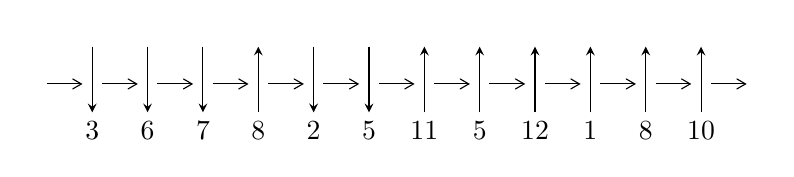
\begin{tikzpicture}[x=20pt, y=17pt]
	% nodes
	\node (C0) at (0, 0) {};
	\node (C1) at (1, 0) {};
	\node (C1U) at (1, +1) {};
	\node (C1D) at (1, -1) {3};

	\node (C2) at (2, 0) {};
	\node (C2U) at (2, +1) {};
	\node (C2D) at (2, -1) {6};

	\node (C3) at (3, 0) {};
	\node (C3U) at (3, +1) {};
	\node (C3D) at (3, -1) {7};

	\node (C4) at (4, 0) {};
	\node (C4U) at (4, +1) {};
	\node (C4D) at (4, -1) {8};

	\node (C5) at (5, 0) {};
	\node (C5U) at (5, +1) {};
	\node (C5D) at (5, -1) {2};

	\node (C6) at (6, 0) {};
	\node (C6U) at (6, +1) {};
	\node (C6D) at (6, -1) {5};

	\node (C7) at (7, 0) {};
	\node (C7U) at (7, +1) {};
	\node (C7D) at (7, -1) {11};

	\node (C8) at (8, 0) {};
	\node (C8U) at (8, +1) {};
	\node (C8D) at (8, -1) {5};

	\node (C9) at (9, 0) {};
	\node (C9U) at (9, +1) {};
	\node (C9D) at (9, -1) {12};

	\node (C10) at (10, 0) {};
	\node (C10U) at (10, +1) {};
	\node (C10D) at (10, -1) {1};

	\node (C11) at (11, 0) {};
	\node (C11U) at (11, +1) {};
	\node (C11D) at (11, -1) {8};

	\node (C12) at (12, 0) {};
	\node (C12U) at (12, +1) {};
	\node (C12D) at (12, -1) {10};
	\node (C13) at (13, 0) {};

	% arrows
	\draw[->,>={angle 60}]
	(C0) edge (C1) (C1) edge (C2) (C2) edge (C3) (C3) edge (C4) (C4) edge (C5) (C5) edge (C6) (C6) edge (C7) (C7) edge (C8) (C8) edge (C9) (C9) edge (C10) (C10) edge (C11) (C11) edge (C12) (C12) edge (C13) ;	\draw[->,>=stealth]
	(C1U) edge (C1D) (C2U) edge (C2D) (C3U) edge (C3D) (C4D) edge (C4U) (C5U) edge (C5D) (C6U) edge (C6D) (C7D) edge (C7U) (C8D) edge (C8U) (C9D) edge (C9U) (C10D) edge (C10U) (C11D) edge (C11U) (C12D) edge (C12U) ;
	\end{tikzpicture} \\
\hhline{~~} \\& 
\textbf{Solving Sequence} \\ \cline{2-2} 
 &
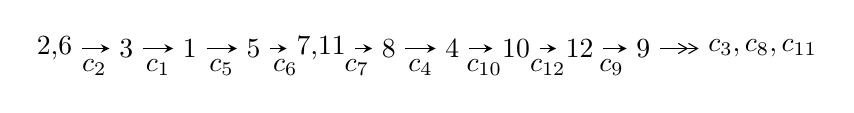
\begin{tikzpicture}[x=23pt, y=7pt]
	% node
	\node (A0) at (-1/8, 0) {2,6};
	\node (A1) at (1, 0) {3};
	\node (A2) at (2, 0) {1};
	\node (A3) at (3, 0) {5};
	\node (A4) at (65/16, 0) {7,11};
	\node (A5) at (41/8, 0) {8};
	\node (A6) at (49/8, 0) {4};
	\node (A7) at (57/8, 0) {10};
	\node (A8) at (65/8, 0) {12};
	\node (A9) at (73/8, 0) {9};
	\node (C1) at (1/2, -1) {$c_{2}$};
	\node (C2) at (3/2, -1) {$c_{1}$};
	\node (C3) at (5/2, -1) {$c_{5}$};
	\node (C4) at (7/2, -1) {$c_{6}$};
	\node (C5) at (37/8, -1) {$c_{7}$};
	\node (C6) at (45/8, -1) {$c_{4}$};
	\node (C7) at (53/8, -1) {$c_{10}$};
	\node (C8) at (61/8, -1) {$c_{12}$};
	\node (C9) at (69/8, -1) {$c_{9}$};
	\node (A10) at (11, 0) {$c_{3},c_{8},c_{11}$};

	% edge
	\draw[->,>=stealth]	
	(A0) edge (A1) (A1) edge (A2) (A2) edge (A3) (A3) edge (A4) (A4) edge (A5) (A5) edge (A6) (A6) edge (A7) (A7) edge (A8) (A8) edge (A9) ;
	\draw[->>,>={angle 60}]	
	(A9) edge (A10);
\end{tikzpicture} \\ 

\end{tabular} \\

\footnotetext{
The image of knot diagram is generated by the software ``\textbf{Draw programme}" developed by Andrew Bartholomew(\url{http://www.layer8.co.uk/maths/draw/index.htm\#Running-draw}), where we modified some parts for our purpose(\url{https://github.com/CATsTAILs/LinksPainter}).
}\phantom \\ \newline 
\centering \textbf{Ideals for irreducible components\footnotemark of $X_{\text{par}}$} 
 
\begin{align*}
I^u_{1}&=\langle 
2.93542\times10^{17} u^{55}-6.67587\times10^{17} u^{54}+\cdots+2.93396\times10^{17} b-4.34022\times10^{16},\\
\phantom{I^u_{1}}&\phantom{= \langle  }2.00229\times10^{18} u^{55}-6.17396\times10^{18} u^{54}+\cdots+2.93396\times10^{17} a-3.02275\times10^{18},\;u^{56}-4 u^{55}+\cdots+2 u+1\rangle \\
I^u_{2}&=\langle 
- u^2 a+u^2+b,\;2 u^2 a+a^2+a u-2 u^2- a-2 u-1,\;u^3+u^2-1\rangle \\
I^u_{3}&=\langle 
b,\;a-1,\;u-1\rangle \\
\\
\end{align*}
\raggedright * 3 irreducible components of $\dim_{\mathbb{C}}=0$, with total 63 representations.\\
\footnotetext{All coefficients of polynomials are rational numbers. But the coefficients are sometimes approximated in decimal forms when there is not enough margin.}
\newpage
\renewcommand{\arraystretch}{1}
\centering \section*{I. $I^u_{1}= \langle 2.94\times10^{17} u^{55}-6.68\times10^{17} u^{54}+\cdots+2.93\times10^{17} b-4.34\times10^{16},\;2.00\times10^{18} u^{55}-6.17\times10^{18} u^{54}+\cdots+2.93\times10^{17} a-3.02\times10^{18},\;u^{56}-4 u^{55}+\cdots+2 u+1 \rangle$}
\flushleft \textbf{(i) Arc colorings}\\
\begin{tabular}{m{7pt} m{180pt} m{7pt} m{180pt} }
\flushright $a_{2}=$&$\begin{pmatrix}1\\0\end{pmatrix}$ \\
\flushright $a_{6}=$&$\begin{pmatrix}0\\u\end{pmatrix}$ \\
\flushright $a_{3}=$&$\begin{pmatrix}1\\u^2\end{pmatrix}$ \\
\flushright $a_{1}=$&$\begin{pmatrix}- u^2+1\\- u^4\end{pmatrix}$ \\
\flushright $a_{5}=$&$\begin{pmatrix}u\\u\end{pmatrix}$ \\
\flushright $a_{7}=$&$\begin{pmatrix}- u^3\\- u^3+u\end{pmatrix}$ \\
\flushright $a_{11}=$&$\begin{pmatrix}-6.82450 u^{55}+21.0431 u^{54}+\cdots+1.50746 u+10.3026\\-1.00050 u^{55}+2.27537 u^{54}+\cdots-2.44477 u+0.147930\end{pmatrix}$ \\
\flushright $a_{8}=$&$\begin{pmatrix}3.65406 u^{55}-10.3520 u^{54}+\cdots+5.15325 u-4.23694\\4.10204 u^{55}-12.0354 u^{54}+\cdots-2.31411 u-2.32151\end{pmatrix}$ \\
\flushright $a_{4}=$&$\begin{pmatrix}- u^8+u^6- u^4+1\\- u^8+2 u^6-2 u^4+2 u^2\end{pmatrix}$ \\
\flushright $a_{10}=$&$\begin{pmatrix}-6.34999 u^{55}+19.7941 u^{54}+\cdots-0.691497 u+9.35095\\-0.586914 u^{55}+1.14134 u^{54}+\cdots-2.44719 u+0.0395175\end{pmatrix}$ \\
\flushright $a_{12}=$&$\begin{pmatrix}-2.57455 u^{55}+8.57238 u^{54}+\cdots-0.0350557 u+6.04787\\3.43407 u^{55}-10.9313 u^{54}+\cdots-6.20880 u-2.54966\end{pmatrix}$ \\
\flushright $a_{9}=$&$\begin{pmatrix}-3.42363 u^{55}+10.3054 u^{54}+\cdots-4.48816 u+4.34550\\-3.87161 u^{55}+11.9888 u^{54}+\cdots+2.97921 u+2.43006\end{pmatrix}$\\&\end{tabular}
\flushleft \textbf{(ii) Obstruction class $= -1$}\\~\\
\flushleft \textbf{(iii) Cusp Shapes $= -\frac{6957411366946544141}{146698213939434107} u^{55}+\frac{43997122065882996801}{293396427878868214} u^{54}+\cdots+\frac{49895915246887856523}{293396427878868214} u+\frac{19684211583463159307}{293396427878868214}$}\\~\\
\newpage\renewcommand{\arraystretch}{1}
\flushleft \textbf{(iv) u-Polynomials at the component}\newline \\
\begin{tabular}{m{50pt}|m{274pt}}
Crossings & \hspace{64pt}u-Polynomials at each crossing \\
\hline $$\begin{aligned}c_{1},c_{6}\end{aligned}$$&$\begin{aligned}
&u^{56}+20 u^{55}+\cdots+94 u+1
\end{aligned}$\\
\hline $$\begin{aligned}c_{2},c_{5}\end{aligned}$$&$\begin{aligned}
&u^{56}+4 u^{55}+\cdots-2 u+1
\end{aligned}$\\
\hline $$\begin{aligned}c_{3}\end{aligned}$$&$\begin{aligned}
&u^{56}-2 u^{55}+\cdots-37222 u+7489
\end{aligned}$\\
\hline $$\begin{aligned}c_{4},c_{8}\end{aligned}$$&$\begin{aligned}
&u^{56}+4 u^{55}+\cdots+416 u-64
\end{aligned}$\\
\hline $$\begin{aligned}c_{7},c_{11}\end{aligned}$$&$\begin{aligned}
&u^{56}-4 u^{55}+\cdots-2 u-2
\end{aligned}$\\
\hline $$\begin{aligned}c_{9},c_{10},c_{12}\end{aligned}$$&$\begin{aligned}
&u^{56}+5 u^{55}+\cdots+3 u+1
\end{aligned}$\\
\hline
\end{tabular}\\~\\
\newpage\renewcommand{\arraystretch}{1}
\flushleft \textbf{(v) Riley Polynomials at the component}\newline \\
\begin{tabular}{m{50pt}|m{274pt}}
Crossings & \hspace{64pt}Riley Polynomials at each crossing \\
\hline $$\begin{aligned}c_{1},c_{6}\end{aligned}$$&$\begin{aligned}
&y^{56}+36 y^{55}+\cdots-6302 y+1
\end{aligned}$\\
\hline $$\begin{aligned}c_{2},c_{5}\end{aligned}$$&$\begin{aligned}
&y^{56}-20 y^{55}+\cdots-94 y+1
\end{aligned}$\\
\hline $$\begin{aligned}c_{3}\end{aligned}$$&$\begin{aligned}
&y^{56}-24 y^{55}+\cdots-5793307970 y+56085121
\end{aligned}$\\
\hline $$\begin{aligned}c_{4},c_{8}\end{aligned}$$&$\begin{aligned}
&y^{56}+34 y^{55}+\cdots-21504 y+4096
\end{aligned}$\\
\hline $$\begin{aligned}c_{7},c_{11}\end{aligned}$$&$\begin{aligned}
&y^{56}-18 y^{55}+\cdots-80 y+4
\end{aligned}$\\
\hline $$\begin{aligned}c_{9},c_{10},c_{12}\end{aligned}$$&$\begin{aligned}
&y^{56}-47 y^{55}+\cdots-71 y+1
\end{aligned}$\\
\hline
\end{tabular}\\~\\
\newpage\flushleft \textbf{(vi) Complex Volumes and Cusp Shapes}
$$\begin{array}{c|c|c}  
\text{Solutions to }I^u_{1}& \I (\text{vol} + \sqrt{-1}CS) & \text{Cusp shape}\\
 \hline 
\begin{aligned}
u &= -0.555632 + 0.820839 I \\
a &= -1.310140 + 0.452763 I \\
b &= -0.50995 + 1.32573 I\end{aligned}
 & \phantom{-}6.89840 - 1.70687 I & \phantom{-}11.04654 + 2.11039 I \\ \hline\begin{aligned}
u &= -0.555632 - 0.820839 I \\
a &= -1.310140 - 0.452763 I \\
b &= -0.50995 - 1.32573 I\end{aligned}
 & \phantom{-}6.89840 + 1.70687 I & \phantom{-}11.04654 - 2.11039 I \\ \hline\begin{aligned}
u &= -0.746093 + 0.643224 I \\
a &= \phantom{-}1.79687 - 0.81232 I \\
b &= \phantom{-}0.61922 - 1.61203 I\end{aligned}
 & \phantom{-}2.14654 + 0.63049 I & \phantom{-}4.81685 + 0. I\phantom{ +0.000000I} \\ \hline\begin{aligned}
u &= -0.746093 - 0.643224 I \\
a &= \phantom{-}1.79687 + 0.81232 I \\
b &= \phantom{-}0.61922 + 1.61203 I\end{aligned}
 & \phantom{-}2.14654 - 0.63049 I & \phantom{-}4.81685 + 0. I\phantom{ +0.000000I} \\ \hline\begin{aligned}
u &= \phantom{-}0.611315 + 0.811190 I \\
a &= \phantom{-}0.82986 + 1.25644 I \\
b &= -0.84573 + 1.32108 I\end{aligned}
 & -1.11438 + 4.39097 I & \phantom{-}2.00000 - 3.05982 I \\ \hline\begin{aligned}
u &= \phantom{-}0.611315 - 0.811190 I \\
a &= \phantom{-}0.82986 - 1.25644 I \\
b &= -0.84573 - 1.32108 I\end{aligned}
 & -1.11438 - 4.39097 I & \phantom{-}2.00000 + 3.05982 I \\ \hline\begin{aligned}
u &= \phantom{-}0.639496 + 0.745500 I \\
a &= \phantom{-}0.21432 + 1.59797 I \\
b &= -0.18371 + 1.40658 I\end{aligned}
 & \phantom{-}2.28095 + 2.17813 I & \phantom{-}5.60335 - 1.04644 I \\ \hline\begin{aligned}
u &= \phantom{-}0.639496 - 0.745500 I \\
a &= \phantom{-}0.21432 - 1.59797 I \\
b &= -0.18371 - 1.40658 I\end{aligned}
 & \phantom{-}2.28095 - 2.17813 I & \phantom{-}5.60335 + 1.04644 I \\ \hline\begin{aligned}
u &= -1.057330 + 0.031394 I \\
a &= \phantom{-}1.059980 + 0.396752 I \\
b &= \phantom{-}1.037210 - 0.754122 I\end{aligned}
 & -3.27157 + 1.64123 I & \phantom{-0.000000 } 0 \\ \hline\begin{aligned}
u &= -1.057330 - 0.031394 I \\
a &= \phantom{-}1.059980 - 0.396752 I \\
b &= \phantom{-}1.037210 + 0.754122 I\end{aligned}
 & -3.27157 - 1.64123 I & \phantom{-0.000000 } 0\\
 \hline 
 \end{array}$$\newpage$$\begin{array}{c|c|c}  
\text{Solutions to }I^u_{1}& \I (\text{vol} + \sqrt{-1}CS) & \text{Cusp shape}\\
 \hline 
\begin{aligned}
u &= -0.815754 + 0.715389 I \\
a &= \phantom{-}2.13178 - 1.95768 I \\
b &= \phantom{-}0.80101 - 3.45506 I\end{aligned}
 & \phantom{-}4.64235 + 1.91730 I & \phantom{-0.000000 } 0 \\ \hline\begin{aligned}
u &= -0.815754 - 0.715389 I \\
a &= \phantom{-}2.13178 + 1.95768 I \\
b &= \phantom{-}0.80101 + 3.45506 I\end{aligned}
 & \phantom{-}4.64235 - 1.91730 I & \phantom{-0.000000 } 0 \\ \hline\begin{aligned}
u &= \phantom{-}0.646892 + 0.638776 I \\
a &= -0.850743 - 0.918967 I \\
b &= \phantom{-}0.826318 - 0.495030 I\end{aligned}
 & \phantom{-}1.49600 - 0.77880 I & \phantom{-}5.52001 + 0.97967 I \\ \hline\begin{aligned}
u &= \phantom{-}0.646892 - 0.638776 I \\
a &= -0.850743 + 0.918967 I \\
b &= \phantom{-}0.826318 + 0.495030 I\end{aligned}
 & \phantom{-}1.49600 + 0.77880 I & \phantom{-}5.52001 - 0.97967 I \\ \hline\begin{aligned}
u &= \phantom{-}0.655547 + 0.884678 I \\
a &= -1.01004 - 1.55997 I \\
b &= \phantom{-}0.57473 - 1.83740 I\end{aligned}
 & \phantom{-}3.85590 + 9.25734 I & \phantom{-0.000000 } 0 \\ \hline\begin{aligned}
u &= \phantom{-}0.655547 - 0.884678 I \\
a &= -1.01004 + 1.55997 I \\
b &= \phantom{-}0.57473 + 1.83740 I\end{aligned}
 & \phantom{-}3.85590 - 9.25734 I & \phantom{-0.000000 } 0 \\ \hline\begin{aligned}
u &= \phantom{-}0.859653 + 0.688129 I \\
a &= \phantom{-}0.664066 - 0.017009 I \\
b &= -0.054388 - 0.658388 I\end{aligned}
 & \phantom{-}11.29430 - 2.64795 I & \phantom{-0.000000 } 0 \\ \hline\begin{aligned}
u &= \phantom{-}0.859653 - 0.688129 I \\
a &= \phantom{-}0.664066 + 0.017009 I \\
b &= -0.054388 + 0.658388 I\end{aligned}
 & \phantom{-}11.29430 + 2.64795 I & \phantom{-0.000000 } 0 \\ \hline\begin{aligned}
u &= \phantom{-}0.876983 + 0.151494 I \\
a &= \phantom{-}0.1160180 + 0.0212256 I \\
b &= -0.393762 - 0.405166 I\end{aligned}
 & -1.49543 - 0.33054 I & -5.58521 + 0.41922 I \\ \hline\begin{aligned}
u &= \phantom{-}0.876983 - 0.151494 I \\
a &= \phantom{-}0.1160180 - 0.0212256 I \\
b &= -0.393762 + 0.405166 I\end{aligned}
 & -1.49543 + 0.33054 I & -5.58521 - 0.41922 I\\
 \hline 
 \end{array}$$\newpage$$\begin{array}{c|c|c}  
\text{Solutions to }I^u_{1}& \I (\text{vol} + \sqrt{-1}CS) & \text{Cusp shape}\\
 \hline 
\begin{aligned}
u &= -1.115310 + 0.073858 I \\
a &= -0.302761 + 0.507491 I \\
b &= -0.541213 - 0.678094 I\end{aligned}
 & -7.34462 + 3.52834 I & \phantom{-0.000000 } 0 \\ \hline\begin{aligned}
u &= -1.115310 - 0.073858 I \\
a &= -0.302761 - 0.507491 I \\
b &= -0.541213 + 0.678094 I\end{aligned}
 & -7.34462 - 3.52834 I & \phantom{-0.000000 } 0 \\ \hline\begin{aligned}
u &= -0.947166 + 0.640358 I \\
a &= -1.40216 + 1.01867 I \\
b &= -0.74124 + 2.06542 I\end{aligned}
 & \phantom{-}1.51907 + 4.39807 I & \phantom{-0.000000 } 0 \\ \hline\begin{aligned}
u &= -0.947166 - 0.640358 I \\
a &= -1.40216 - 1.01867 I \\
b &= -0.74124 - 2.06542 I\end{aligned}
 & \phantom{-}1.51907 - 4.39807 I & \phantom{-0.000000 } 0 \\ \hline\begin{aligned}
u &= -0.904546 + 0.704031 I \\
a &= -2.66914 + 2.18937 I \\
b &= -0.75000 + 3.34742 I\end{aligned}
 & \phantom{-}4.37132 + 3.51272 I & \phantom{-0.000000 } 0 \\ \hline\begin{aligned}
u &= -0.904546 - 0.704031 I \\
a &= -2.66914 - 2.18937 I \\
b &= -0.75000 - 3.34742 I\end{aligned}
 & \phantom{-}4.37132 - 3.51272 I & \phantom{-0.000000 } 0 \\ \hline\begin{aligned}
u &= \phantom{-}0.199557 + 0.823827 I \\
a &= -0.188450 + 0.800184 I \\
b &= -0.896805 - 0.162123 I\end{aligned}
 & \phantom{-}1.27100 - 5.53243 I & \phantom{-}6.88478 + 5.95128 I \\ \hline\begin{aligned}
u &= \phantom{-}0.199557 - 0.823827 I \\
a &= -0.188450 - 0.800184 I \\
b &= -0.896805 + 0.162123 I\end{aligned}
 & \phantom{-}1.27100 + 5.53243 I & \phantom{-}6.88478 - 5.95128 I \\ \hline\begin{aligned}
u &= -1.149520 + 0.171385 I \\
a &= -0.352409 - 0.425484 I \\
b &= \phantom{-}0.086994 + 0.749495 I\end{aligned}
 & -3.37562 + 8.61142 I & \phantom{-0.000000 } 0 \\ \hline\begin{aligned}
u &= -1.149520 - 0.171385 I \\
a &= -0.352409 + 0.425484 I \\
b &= \phantom{-}0.086994 - 0.749495 I\end{aligned}
 & -3.37562 - 8.61142 I & \phantom{-0.000000 } 0\\
 \hline 
 \end{array}$$\newpage$$\begin{array}{c|c|c}  
\text{Solutions to }I^u_{1}& \I (\text{vol} + \sqrt{-1}CS) & \text{Cusp shape}\\
 \hline 
\begin{aligned}
u &= -0.877750 + 0.767459 I \\
a &= \phantom{-}0.61912 + 1.30040 I \\
b &= \phantom{-}1.71436 + 0.44120 I\end{aligned}
 & \phantom{-}3.73144 + 2.89531 I & \phantom{-0.000000 } 0 \\ \hline\begin{aligned}
u &= -0.877750 - 0.767459 I \\
a &= \phantom{-}0.61912 - 1.30040 I \\
b &= \phantom{-}1.71436 - 0.44120 I\end{aligned}
 & \phantom{-}3.73144 - 2.89531 I & \phantom{-0.000000 } 0 \\ \hline\begin{aligned}
u &= \phantom{-}0.996417 + 0.644457 I \\
a &= \phantom{-}1.098620 - 0.312059 I \\
b &= \phantom{-}1.46572 + 1.16153 I\end{aligned}
 & \phantom{-}0.45076 - 4.30103 I & \phantom{-0.000000 } 0 \\ \hline\begin{aligned}
u &= \phantom{-}0.996417 - 0.644457 I \\
a &= \phantom{-}1.098620 + 0.312059 I \\
b &= \phantom{-}1.46572 - 1.16153 I\end{aligned}
 & \phantom{-}0.45076 + 4.30103 I & \phantom{-0.000000 } 0 \\ \hline\begin{aligned}
u &= \phantom{-}0.807123\phantom{ +0.000000I} \\
a &= \phantom{-}3.25049\phantom{ +0.000000I} \\
b &= -1.20792\phantom{ +0.000000I}\end{aligned}
 & \phantom{-}0.339779\phantom{ +0.000000I} & \phantom{-}61.8040\phantom{ +0.000000I} \\ \hline\begin{aligned}
u &= \phantom{-}1.041510 + 0.583028 I \\
a &= \phantom{-}1.391730 - 0.045593 I \\
b &= \phantom{-}1.52856 + 0.47260 I\end{aligned}
 & -4.20570 - 3.27627 I & \phantom{-0.000000 } 0 \\ \hline\begin{aligned}
u &= \phantom{-}1.041510 - 0.583028 I \\
a &= \phantom{-}1.391730 + 0.045593 I \\
b &= \phantom{-}1.52856 - 0.47260 I\end{aligned}
 & -4.20570 + 3.27627 I & \phantom{-0.000000 } 0 \\ \hline\begin{aligned}
u &= \phantom{-}0.386849 + 0.703387 I \\
a &= \phantom{-}0.080082 - 1.229030 I \\
b &= \phantom{-}0.502755 - 0.488230 I\end{aligned}
 & -2.39037 - 1.55268 I & \phantom{-}1.61575 + 2.61232 I \\ \hline\begin{aligned}
u &= \phantom{-}0.386849 - 0.703387 I \\
a &= \phantom{-}0.080082 + 1.229030 I \\
b &= \phantom{-}0.502755 + 0.488230 I\end{aligned}
 & -2.39037 + 1.55268 I & \phantom{-}1.61575 - 2.61232 I \\ \hline\begin{aligned}
u &= \phantom{-}1.115730 + 0.439932 I \\
a &= -0.739493 + 0.517959 I \\
b &= -1.131660 + 0.027778 I\end{aligned}
 & -1.67584 + 0.98983 I & \phantom{-0.000000 } 0\\
 \hline 
 \end{array}$$\newpage$$\begin{array}{c|c|c}  
\text{Solutions to }I^u_{1}& \I (\text{vol} + \sqrt{-1}CS) & \text{Cusp shape}\\
 \hline 
\begin{aligned}
u &= \phantom{-}1.115730 - 0.439932 I \\
a &= -0.739493 - 0.517959 I \\
b &= -1.131660 - 0.027778 I\end{aligned}
 & -1.67584 - 0.98983 I & \phantom{-0.000000 } 0 \\ \hline\begin{aligned}
u &= \phantom{-}1.21660\phantom{ +0.000000I} \\
a &= -0.482061\phantom{ +0.000000I} \\
b &= \phantom{-}0.154807\phantom{ +0.000000I}\end{aligned}
 & \phantom{-}0.661022\phantom{ +0.000000I} & \phantom{-0.000000 } 0 \\ \hline\begin{aligned}
u &= \phantom{-}1.013820 + 0.677594 I \\
a &= -1.87407 - 0.28208 I \\
b &= -1.80895 - 0.83661 I\end{aligned}
 & \phantom{-}1.16708 - 7.61471 I & \phantom{-0.000000 } 0 \\ \hline\begin{aligned}
u &= \phantom{-}1.013820 - 0.677594 I \\
a &= -1.87407 + 0.28208 I \\
b &= -1.80895 + 0.83661 I\end{aligned}
 & \phantom{-}1.16708 + 7.61471 I & \phantom{-0.000000 } 0 \\ \hline\begin{aligned}
u &= \phantom{-}1.043410 + 0.693114 I \\
a &= -1.80141 - 0.10454 I \\
b &= -1.81609 - 1.65261 I\end{aligned}
 & -2.41199 - 10.04440 I & \phantom{-0.000000 } 0 \\ \hline\begin{aligned}
u &= \phantom{-}1.043410 - 0.693114 I \\
a &= -1.80141 + 0.10454 I \\
b &= -1.81609 + 1.65261 I\end{aligned}
 & -2.41199 + 10.04440 I & \phantom{-0.000000 } 0 \\ \hline\begin{aligned}
u &= -1.063310 + 0.686319 I \\
a &= \phantom{-}1.20482 - 1.11113 I \\
b &= \phantom{-}0.57272 - 1.88306 I\end{aligned}
 & \phantom{-}5.39990 + 7.34868 I & \phantom{-0.000000 } 0 \\ \hline\begin{aligned}
u &= -1.063310 - 0.686319 I \\
a &= \phantom{-}1.20482 + 1.11113 I \\
b &= \phantom{-}0.57272 + 1.88306 I\end{aligned}
 & \phantom{-}5.39990 - 7.34868 I & \phantom{-0.000000 } 0 \\ \hline\begin{aligned}
u &= -0.906500 + 0.883744 I \\
a &= \phantom{-}0.426122 + 0.260836 I \\
b &= \phantom{-}0.259723 + 0.288378 I\end{aligned}
 & \phantom{-}8.38533 + 3.24583 I & \phantom{-0.000000 } 0 \\ \hline\begin{aligned}
u &= -0.906500 - 0.883744 I \\
a &= \phantom{-}0.426122 - 0.260836 I \\
b &= \phantom{-}0.259723 - 0.288378 I\end{aligned}
 & \phantom{-}8.38533 - 3.24583 I & \phantom{-0.000000 } 0\\
 \hline 
 \end{array}$$\newpage$$\begin{array}{c|c|c}  
\text{Solutions to }I^u_{1}& \I (\text{vol} + \sqrt{-1}CS) & \text{Cusp shape}\\
 \hline 
\begin{aligned}
u &= \phantom{-}1.055930 + 0.737690 I \\
a &= \phantom{-}2.11012 + 0.58896 I \\
b &= \phantom{-}1.89812 + 2.08623 I\end{aligned}
 & \phantom{-}2.6209 - 15.2730 I & \phantom{-0.000000 } 0 \\ \hline\begin{aligned}
u &= \phantom{-}1.055930 - 0.737690 I \\
a &= \phantom{-}2.11012 - 0.58896 I \\
b &= \phantom{-}1.89812 - 2.08623 I\end{aligned}
 & \phantom{-}2.6209 + 15.2730 I & \phantom{-0.000000 } 0 \\ \hline\begin{aligned}
u &= -0.665378\phantom{ +0.000000I} \\
a &= -2.70313\phantom{ +0.000000I} \\
b &= -1.90693\phantom{ +0.000000I}\end{aligned}
 & \phantom{-}7.93809\phantom{ +0.000000I} & \phantom{-}29.4940\phantom{ +0.000000I} \\ \hline\begin{aligned}
u &= \phantom{-}0.372658 + 0.279589 I \\
a &= -1.53134 - 0.64420 I \\
b &= \phantom{-}1.017650 - 0.002132 I\end{aligned}
 & \phantom{-}1.155810 - 0.800051 I & \phantom{-}6.92184 - 0.19721 I \\ \hline\begin{aligned}
u &= \phantom{-}0.372658 - 0.279589 I \\
a &= -1.53134 + 0.64420 I \\
b &= \phantom{-}1.017650 + 0.002132 I\end{aligned}
 & \phantom{-}1.155810 + 0.800051 I & \phantom{-}6.92184 + 0.19721 I \\ \hline\begin{aligned}
u &= -0.112048\phantom{ +0.000000I} \\
a &= \phantom{-}5.51199\phantom{ +0.000000I} \\
b &= \phantom{-}0.496888\phantom{ +0.000000I}\end{aligned}
 & \phantom{-}0.859867\phantom{ +0.000000I} & \phantom{-}11.9670\phantom{ +0.000000I}\\
 \hline 
 \end{array}$$\newpage\newpage\renewcommand{\arraystretch}{1}
\centering \section*{II. $I^u_{2}= \langle - u^2 a+u^2+b,\;2 u^2 a+a^2+a u-2 u^2- a-2 u-1,\;u^3+u^2-1 \rangle$}
\flushleft \textbf{(i) Arc colorings}\\
\begin{tabular}{m{7pt} m{180pt} m{7pt} m{180pt} }
\flushright $a_{2}=$&$\begin{pmatrix}1\\0\end{pmatrix}$ \\
\flushright $a_{6}=$&$\begin{pmatrix}0\\u\end{pmatrix}$ \\
\flushright $a_{3}=$&$\begin{pmatrix}1\\u^2\end{pmatrix}$ \\
\flushright $a_{1}=$&$\begin{pmatrix}- u^2+1\\- u^2- u+1\end{pmatrix}$ \\
\flushright $a_{5}=$&$\begin{pmatrix}u\\u\end{pmatrix}$ \\
\flushright $a_{7}=$&$\begin{pmatrix}u^2-1\\u^2+u-1\end{pmatrix}$ \\
\flushright $a_{11}=$&$\begin{pmatrix}a\\u^2 a- u^2\end{pmatrix}$ \\
\flushright $a_{8}=$&$\begin{pmatrix}- a u+2 u^2+2 u-1\\- a u+2 u^2+2 u-1\end{pmatrix}$ \\
\flushright $a_{4}=$&$\begin{pmatrix}u\\u\end{pmatrix}$ \\
\flushright $a_{10}=$&$\begin{pmatrix}a u-2 u^2- u+2\\a u-2 u^2-2 u+2\end{pmatrix}$ \\
\flushright $a_{12}=$&$\begin{pmatrix}-2 a u+3 u^2+a+3 u-2\\u^2 a-2 a u+2 u^2+3 u-2\end{pmatrix}$ \\
\flushright $a_{9}=$&$\begin{pmatrix}- a u+2 u^2+2 u-1\\- a u+2 u^2+2 u-1\end{pmatrix}$\\&\end{tabular}
\flushleft \textbf{(ii) Obstruction class $= 1$}\\~\\
\flushleft \textbf{(iii) Cusp Shapes $= 3 u^2 a-4 u^2+3 a-10 u+3$}\\~\\
\newpage\renewcommand{\arraystretch}{1}
\flushleft \textbf{(iv) u-Polynomials at the component}\newline \\
\begin{tabular}{m{50pt}|m{274pt}}
Crossings & \hspace{64pt}u-Polynomials at each crossing \\
\hline $$\begin{aligned}c_{1},c_{3}\end{aligned}$$&$\begin{aligned}
&(u^3- u^2+2 u-1)^2
\end{aligned}$\\
\hline $$\begin{aligned}c_{2}\end{aligned}$$&$\begin{aligned}
&(u^3+u^2-1)^2
\end{aligned}$\\
\hline $$\begin{aligned}c_{4},c_{8}\end{aligned}$$&$\begin{aligned}
&u^6
\end{aligned}$\\
\hline $$\begin{aligned}c_{5}\end{aligned}$$&$\begin{aligned}
&(u^3- u^2+1)^2
\end{aligned}$\\
\hline $$\begin{aligned}c_{6}\end{aligned}$$&$\begin{aligned}
&(u^3+u^2+2 u+1)^2
\end{aligned}$\\
\hline $$\begin{aligned}c_{7},c_{9},c_{10}\end{aligned}$$&$\begin{aligned}
&(u^2- u-1)^3
\end{aligned}$\\
\hline $$\begin{aligned}c_{11},c_{12}\end{aligned}$$&$\begin{aligned}
&(u^2+u-1)^3
\end{aligned}$\\
\hline
\end{tabular}\\~\\
\newpage\renewcommand{\arraystretch}{1}
\flushleft \textbf{(v) Riley Polynomials at the component}\newline \\
\begin{tabular}{m{50pt}|m{274pt}}
Crossings & \hspace{64pt}Riley Polynomials at each crossing \\
\hline $$\begin{aligned}c_{1},c_{3},c_{6}\end{aligned}$$&$\begin{aligned}
&(y^3+3 y^2+2 y-1)^2
\end{aligned}$\\
\hline $$\begin{aligned}c_{2},c_{5}\end{aligned}$$&$\begin{aligned}
&(y^3- y^2+2 y-1)^2
\end{aligned}$\\
\hline $$\begin{aligned}c_{4},c_{8}\end{aligned}$$&$\begin{aligned}
&y^6
\end{aligned}$\\
\hline $$\begin{aligned}c_{7},c_{9},c_{10}\\c_{11},c_{12}\end{aligned}$$&$\begin{aligned}
&(y^2-3 y+1)^3
\end{aligned}$\\
\hline
\end{tabular}\\~\\
\newpage\flushleft \textbf{(vi) Complex Volumes and Cusp Shapes}
$$\begin{array}{c|c|c}  
\text{Solutions to }I^u_{2}& \I (\text{vol} + \sqrt{-1}CS) & \text{Cusp shape}\\
 \hline 
\begin{aligned}
u &= -0.877439 + 0.744862 I \\
a &= \phantom{-}0.586612 + 0.101930 I \\
b &= \phantom{-}0.044325 + 0.562280 I\end{aligned}
 & \phantom{-}11.90680 + 2.82812 I & \phantom{-}13.45212 - 4.14885 I \\ \hline\begin{aligned}
u &= -0.877439 + 0.744862 I \\
a &= \phantom{-}0.86067 + 1.76749 I \\
b &= \phantom{-}2.28039 + 0.56228 I\end{aligned}
 & \phantom{-}4.01109 + 2.82812 I & \phantom{-}20.9825 + 0.8478 I \\ \hline\begin{aligned}
u &= -0.877439 - 0.744862 I \\
a &= \phantom{-}0.586612 - 0.101930 I \\
b &= \phantom{-}0.044325 - 0.562280 I\end{aligned}
 & \phantom{-}11.90680 - 2.82812 I & \phantom{-}13.45212 + 4.14885 I \\ \hline\begin{aligned}
u &= -0.877439 - 0.744862 I \\
a &= \phantom{-}0.86067 - 1.76749 I \\
b &= \phantom{-}2.28039 - 0.56228 I\end{aligned}
 & \phantom{-}4.01109 - 2.82812 I & \phantom{-}20.9825 - 0.8478 I \\ \hline\begin{aligned}
u &= \phantom{-}0.754878\phantom{ +0.000000I} \\
a &= \phantom{-}1.51473\phantom{ +0.000000I} \\
b &= \phantom{-}0.293316\phantom{ +0.000000I}\end{aligned}
 & -0.126494\phantom{ +0.000000I} & \phantom{-}0.305530\phantom{ +0.000000I} \\ \hline\begin{aligned}
u &= \phantom{-}0.754878\phantom{ +0.000000I} \\
a &= -2.40929\phantom{ +0.000000I} \\
b &= -1.94275\phantom{ +0.000000I}\end{aligned}
 & \phantom{-}7.76919\phantom{ +0.000000I} & -18.1750\phantom{ +0.000000I}\\
 \hline 
 \end{array}$$\newpage\newpage\renewcommand{\arraystretch}{1}
\centering \section*{III. $I^u_{3}= \langle b,\;a-1,\;u-1 \rangle$}
\flushleft \textbf{(i) Arc colorings}\\
\begin{tabular}{m{7pt} m{180pt} m{7pt} m{180pt} }
\flushright $a_{2}=$&$\begin{pmatrix}1\\0\end{pmatrix}$ \\
\flushright $a_{6}=$&$\begin{pmatrix}0\\1\end{pmatrix}$ \\
\flushright $a_{3}=$&$\begin{pmatrix}1\\1\end{pmatrix}$ \\
\flushright $a_{1}=$&$\begin{pmatrix}0\\-1\end{pmatrix}$ \\
\flushright $a_{5}=$&$\begin{pmatrix}1\\1\end{pmatrix}$ \\
\flushright $a_{7}=$&$\begin{pmatrix}-1\\0\end{pmatrix}$ \\
\flushright $a_{11}=$&$\begin{pmatrix}1\\0\end{pmatrix}$ \\
\flushright $a_{8}=$&$\begin{pmatrix}-1\\0\end{pmatrix}$ \\
\flushright $a_{4}=$&$\begin{pmatrix}0\\1\end{pmatrix}$ \\
\flushright $a_{10}=$&$\begin{pmatrix}1\\1\end{pmatrix}$ \\
\flushright $a_{12}=$&$\begin{pmatrix}1\\0\end{pmatrix}$ \\
\flushright $a_{9}=$&$\begin{pmatrix}0\\1\end{pmatrix}$\\&\end{tabular}
\flushleft \textbf{(ii) Obstruction class $= 1$}\\~\\
\flushleft \textbf{(iii) Cusp Shapes $= 0$}\\~\\
\newpage\renewcommand{\arraystretch}{1}
\flushleft \textbf{(iv) u-Polynomials at the component}\newline \\
\begin{tabular}{m{50pt}|m{274pt}}
Crossings & \hspace{64pt}u-Polynomials at each crossing \\
\hline $$\begin{aligned}c_{1},c_{2},c_{3}\\c_{4},c_{12}\end{aligned}$$&$\begin{aligned}
&u-1
\end{aligned}$\\
\hline $$\begin{aligned}c_{5},c_{6},c_{8}\\c_{9},c_{10}\end{aligned}$$&$\begin{aligned}
&u+1
\end{aligned}$\\
\hline $$\begin{aligned}c_{7},c_{11}\end{aligned}$$&$\begin{aligned}
&u
\end{aligned}$\\
\hline
\end{tabular}\\~\\
\newpage\renewcommand{\arraystretch}{1}
\flushleft \textbf{(v) Riley Polynomials at the component}\newline \\
\begin{tabular}{m{50pt}|m{274pt}}
Crossings & \hspace{64pt}Riley Polynomials at each crossing \\
\hline $$\begin{aligned}c_{1},c_{2},c_{3}\\c_{4},c_{5},c_{6}\\c_{8},c_{9},c_{10}\\c_{12}\end{aligned}$$&$\begin{aligned}
&y-1
\end{aligned}$\\
\hline $$\begin{aligned}c_{7},c_{11}\end{aligned}$$&$\begin{aligned}
&y
\end{aligned}$\\
\hline
\end{tabular}\\~\\
\newpage\flushleft \textbf{(vi) Complex Volumes and Cusp Shapes}
$$\begin{array}{c|c|c}  
\text{Solutions to }I^u_{3}& \I (\text{vol} + \sqrt{-1}CS) & \text{Cusp shape}\\
 \hline 
\begin{aligned}
u &= \phantom{-}1.00000\phantom{ +0.000000I} \\
a &= \phantom{-}1.00000\phantom{ +0.000000I} \\
b &= \phantom{-0.000000 } 0\end{aligned}
 & \phantom{-0.000000 } 0 & \phantom{-0.000000 } 0\\
 \hline 
 \end{array}$$\newpage
\newpage\renewcommand{\arraystretch}{1}
\centering \section*{ IV. u-Polynomials}
\begin{tabular}{m{50pt}|m{274pt}}
Crossings & \hspace{64pt}u-Polynomials at each crossing \\
\hline $$\begin{aligned}c_{1}\end{aligned}$$&$\begin{aligned}
&(u-1)(u^3- u^2+2 u-1)^2(u^{56}+20 u^{55}+\cdots+94 u+1)
\end{aligned}$\\
\hline $$\begin{aligned}c_{2}\end{aligned}$$&$\begin{aligned}
&(u-1)(u^3+u^2-1)^2(u^{56}+4 u^{55}+\cdots-2 u+1)
\end{aligned}$\\
\hline $$\begin{aligned}c_{3}\end{aligned}$$&$\begin{aligned}
&(u-1)(u^3- u^2+2 u-1)^2(u^{56}-2 u^{55}+\cdots-37222 u+7489)
\end{aligned}$\\
\hline $$\begin{aligned}c_{4}\end{aligned}$$&$\begin{aligned}
&u^6(u-1)(u^{56}+4 u^{55}+\cdots+416 u-64)
\end{aligned}$\\
\hline $$\begin{aligned}c_{5}\end{aligned}$$&$\begin{aligned}
&(u+1)(u^3- u^2+1)^2(u^{56}+4 u^{55}+\cdots-2 u+1)
\end{aligned}$\\
\hline $$\begin{aligned}c_{6}\end{aligned}$$&$\begin{aligned}
&(u+1)(u^3+u^2+2 u+1)^2(u^{56}+20 u^{55}+\cdots+94 u+1)
\end{aligned}$\\
\hline $$\begin{aligned}c_{7}\end{aligned}$$&$\begin{aligned}
&u(u^2- u-1)^3(u^{56}-4 u^{55}+\cdots-2 u-2)
\end{aligned}$\\
\hline $$\begin{aligned}c_{8}\end{aligned}$$&$\begin{aligned}
&u^6(u+1)(u^{56}+4 u^{55}+\cdots+416 u-64)
\end{aligned}$\\
\hline $$\begin{aligned}c_{9},c_{10}\end{aligned}$$&$\begin{aligned}
&(u+1)(u^2- u-1)^3(u^{56}+5 u^{55}+\cdots+3 u+1)
\end{aligned}$\\
\hline $$\begin{aligned}c_{11}\end{aligned}$$&$\begin{aligned}
&u(u^2+u-1)^3(u^{56}-4 u^{55}+\cdots-2 u-2)
\end{aligned}$\\
\hline $$\begin{aligned}c_{12}\end{aligned}$$&$\begin{aligned}
&(u-1)(u^2+u-1)^3(u^{56}+5 u^{55}+\cdots+3 u+1)
\end{aligned}$\\
\hline
\end{tabular}\newpage\renewcommand{\arraystretch}{1}
\centering \section*{ V. Riley Polynomials}
\begin{tabular}{m{50pt}|m{274pt}}
Crossings & \hspace{64pt}Riley Polynomials at each crossing \\
\hline $$\begin{aligned}c_{1},c_{6}\end{aligned}$$&$\begin{aligned}
&(y-1)(y^3+3 y^2+2 y-1)^2(y^{56}+36 y^{55}+\cdots-6302 y+1)
\end{aligned}$\\
\hline $$\begin{aligned}c_{2},c_{5}\end{aligned}$$&$\begin{aligned}
&(y-1)(y^3- y^2+2 y-1)^2(y^{56}-20 y^{55}+\cdots-94 y+1)
\end{aligned}$\\
\hline $$\begin{aligned}c_{3}\end{aligned}$$&$\begin{aligned}
&(y-1)(y^3+3 y^2+2 y-1)^2\\
&\cdot(y^{56}-24 y^{55}+\cdots-5793307970 y+56085121)
\end{aligned}$\\
\hline $$\begin{aligned}c_{4},c_{8}\end{aligned}$$&$\begin{aligned}
&y^6(y-1)(y^{56}+34 y^{55}+\cdots-21504 y+4096)
\end{aligned}$\\
\hline $$\begin{aligned}c_{7},c_{11}\end{aligned}$$&$\begin{aligned}
&y(y^2-3 y+1)^3(y^{56}-18 y^{55}+\cdots-80 y+4)
\end{aligned}$\\
\hline $$\begin{aligned}c_{9},c_{10},c_{12}\end{aligned}$$&$\begin{aligned}
&(y-1)(y^2-3 y+1)^3(y^{56}-47 y^{55}+\cdots-71 y+1)
\end{aligned}$\\
\hline
\end{tabular}
\vskip 2pc
\end{document}